\documentclass[crop,tikz]{standalone}
\usetikzlibrary{backgrounds}
\colorlet{blue}{cyan}
\tikzset{
  inverted/.style = {
    color=white,
    background rectangle/.style={fill},
    show background rectangle
  }
}

\tikzset{>=latex}

\begin{document}
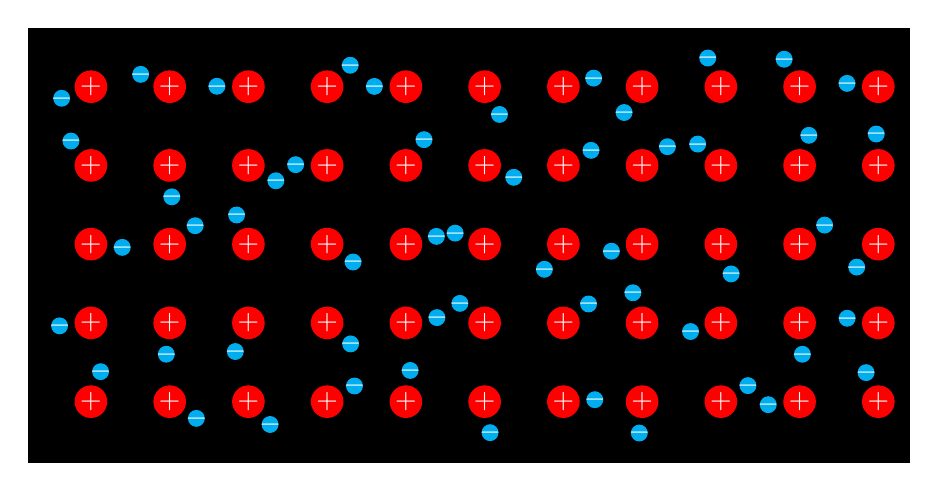
\begin{tikzpicture}[inverted,inverted]
  \foreach \x in { 0,...,10 } {%
    \foreach \y in { 0,...,4 } {%
      \draw[fill,red] (\x,\y) circle (0.2) coordinate (t) node[white] {$+$};
      \draw[fill,blue] (t)++(rand*180:0.4) circle (0.1) node[white] {$-$};
    }
  }
\end{tikzpicture}
\end{document}
